\documentclass[aspectratio=169, xcolor=dvipsnames]{beamer}
\usepackage{basileabeam}
\usepackage{comment}
\usepackage{amsfonts}
\usepackage{mathtools}
\usepackage{xcolor}
\usepackage{amsmath}

% Notes:
%\pgfpagesuselayout{2 on 1}[a4paper,border shrink=5mm]
%\setbeamertemplate{note page}[plain]
%\setbeameroption{show notes on second screen=bottom}

\title              {Mutex Based Potential Heuristics}

\author             {Salome M\"uller}
\email              {salo.mueller@unibas.ch}
\institute          {Department of Mathematics and Computer Science, University of Basel}

\date               {20.11.2020}

\ulogo                {Template/header}
\ulistelement        {Template/listelement}

\graphicspath{{Figures/}}

% Options:
\totalNoSlidesDisabled % To turn off the total number of slides in the footer. Comment this if you want the total number of slides in the footer

%\headerSectionsDisabled % Comment this if you want a fancy header containing your sections.


\begin{document}

    \begin{frame}[t,plain]
        \titlepage
    \end{frame}

    \section{Background}
    \begin{frame}[c]{Classical Planning}
        \begin{itemize}
            \item States $s\in\mathcal{S}$
            \item Facts $f = \langle V, v  \rangle$, $f\in\mathcal{F}$
            \item Operators $o\in\mathcal{O}$
            \begin{itemize}
                \item $\text{cost}(o)$
                \item $\text{pre}(o)\subset\mathcal{F}$
                \item $\text{eff}(o)\subset\mathcal{F}$
            \end{itemize}
            \item Path $\pi$
        \end{itemize}
    \end{frame}

    \begin{frame}[c]{15-Puzzle}
        \begin{figure}
            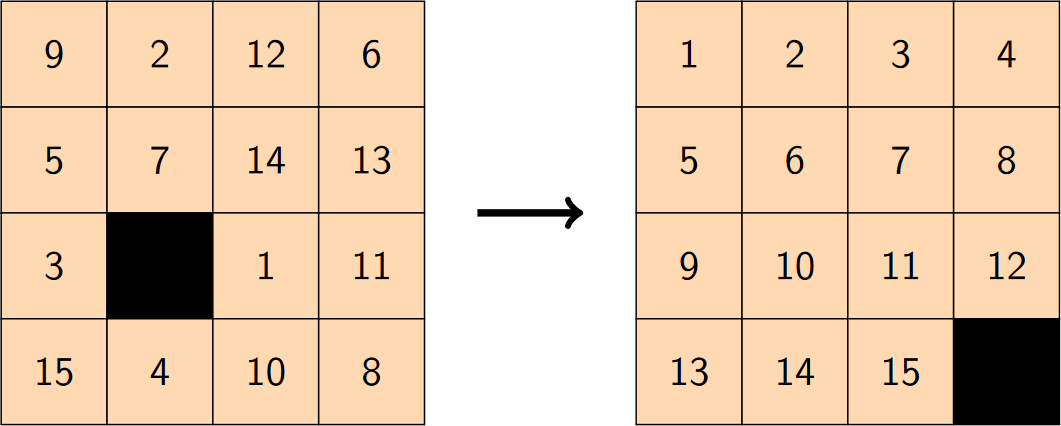
\includegraphics[width=0.8\textwidth]{15-puzzle}
            \footnote{Image from Lecture \textit{Introduction to Artificial Intelligence} (FS 2020)}
        \end{figure}
        \begin{columns}[c]
            \column{.45\textwidth}
            \center Initial State
            \column{.45\textwidth}
            \center Goal State
        \end{columns}
    \end{frame}

    \begin{frame}[c]{Potential Heuristics}
        \begin{definition}[General Heuristic]
            \[h:\mathcal{R} \rightarrow \mathbb{R} \cup \{\infty\}\]
        \end{definition}

        \begin{definition}[Potential Heuristic]
            \[h^\mathtt{P}(s)=\sum_{f\in s}P(f)\]
        \end{definition}
    \end{frame}

    \begin{frame}[c]{Linear Program}
        \begin{itemize}
            \item Optimization Functions
            \begin{itemize}
                \item Linear combination of potentials
                \item Different optimization functions yield different heuristics
            \end{itemize}
            \item Constraints
            \begin{itemize}
                \item Inequalities
                \item Assure admissibility
            \end{itemize}
        \end{itemize}
    \end{frame}

    \begin{frame}[c]{Mutexes and Disambiguations}
        \begin{columns}[c]
            \column{.45\textwidth}
            \begin{tabbing}
                \onslide<1-> Variables: \qquad\qquad\= \textcolor{Cyan}{$A$}, \textcolor{PineGreen}{$B$}, \textcolor{RoyalPurple}{$C$} \\ \\
                \onslide<2-> Domain: \> $\text{dom}(\textcolor{Cyan}{A})=\{1, 2, 3\}$ \\
                \> $\text{dom}(\textcolor{PineGreen}{B})=\{1, 2, 3\}$ \\
                \>$\text{dom}(\textcolor{RoyalPurple}{C})=\{1, 2, 3\}$ \\ \\
                \onslide<4-> Mutex Set: \> $\{$ \= $\{\textcolor{Cyan}{\langle A,1 \rangle}, \textcolor{PineGreen}{\langle B,1 \rangle}\},$ \\
                \onslide<8-> \> \> $\{\textcolor{PineGreen}{\langle B,2 \rangle}, \textcolor{RoyalPurple}{\langle C,3 \rangle}\},$ \\
                \onslide<8-> \> \> $\{\textcolor{PineGreen}{\langle B,3 \rangle}, \textcolor{RoyalPurple}{\langle C,3 \rangle}\}$ $\}$ \\ \\
                \onslide<7-> Disambiguation Set: \> $\{$ \> $\textcolor{PineGreen}{\langle B,2 \rangle}, \textcolor{PineGreen}{\langle B,3 \rangle},$ \\
                \onslide<10>\> \> $\textcolor{RoyalPurple}{\langle C,1 \rangle}, \textcolor{RoyalPurple}{\langle C,2 \rangle}$ $\}$ \\
            \end{tabbing}

            \column{.45\textwidth}
            \begin{centering}
                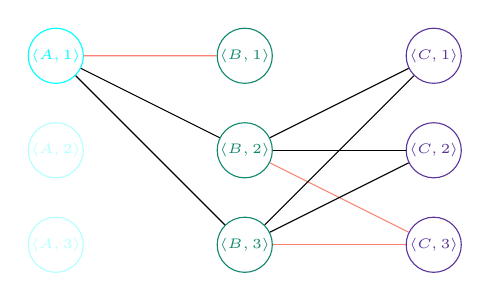
\begin{tikzpicture}
                [every node/.style={circle,inner sep=0pt,minimum size=7mm},scale=0.6]

                    \onslide<3->
                    \node[draw,circle,Cyan]    (A1) at (0,4)    {\tiny $\langle A,1 \rangle$};
                    \node[draw,circle,Cyan,opacity=0.3]    (A2) at (0,2)    {\tiny $\langle A,2 \rangle$};
                    \node[draw,circle,Cyan,opacity=0.3]    (A3) at (0,0)    {\tiny $\langle A,3 \rangle$};

                    \onslide<5->
                    \node[draw,circle,PineGreen]    (B1) at (4,4)    {\tiny $\langle B,1 \rangle$};
                    \draw[-,>=latex,Salmon] (A1) -- (B1);

                    \onslide<6->
                    \node[draw,circle,PineGreen]    (B2) at (4,2)    {\tiny $\langle B,2 \rangle$};
                    \node[draw,circle,PineGreen]    (B3) at (4,0)    {\tiny $\langle B,3 \rangle$};
                    \draw[-,>=latex] (A1) -- (B2);
                    \draw[-,>=latex] (A1) -- (B3);

                    \onslide<9->
                    \node[draw,circle,RoyalPurple]    (C3) at (8,0)    {\tiny $\langle C,3 \rangle$};
                    \draw[-,>=latex,Salmon] (B2) -- (C3);
                    \draw[-,>=latex,Salmon] (B3) -- (C3);

                    \onslide<10->
                    \node[draw,circle,RoyalPurple]    (C1) at (8,4)    {\tiny $\langle C,1 \rangle$};
                    \node[draw,circle,RoyalPurple]    (C2) at (8,2)    {\tiny $\langle C,2 \rangle$};
                    \draw[-,>=latex] (B2) -- (C1);
                    \draw[-,>=latex] (B2) -- (C2);
                    \draw[-,>=latex] (B3) -- (C1);
                    \draw[-,>=latex] (B3) -- (C2);

                \end{tikzpicture}
            \end{centering}
        \end{columns}
    \end{frame}

    \section{Linear Program}
    \begin{frame}[c]{Strengthen LP Constraints}
        \begin{definition}[Constraint for Goal-Awareness]
            \[\sum_{f\in G}\mathtt{P}(f)+\sum_{V\in\mathcal{V}\setminus\mathrm{vars}(G)}\max_{f\in\mathcal{F}_V}\mathtt{P}(f)\leq0 \]
        \end{definition}
    \end{frame}

    \begin{frame}[c]{Strengthen LP Constraints: Results}
        \begin{figure}
            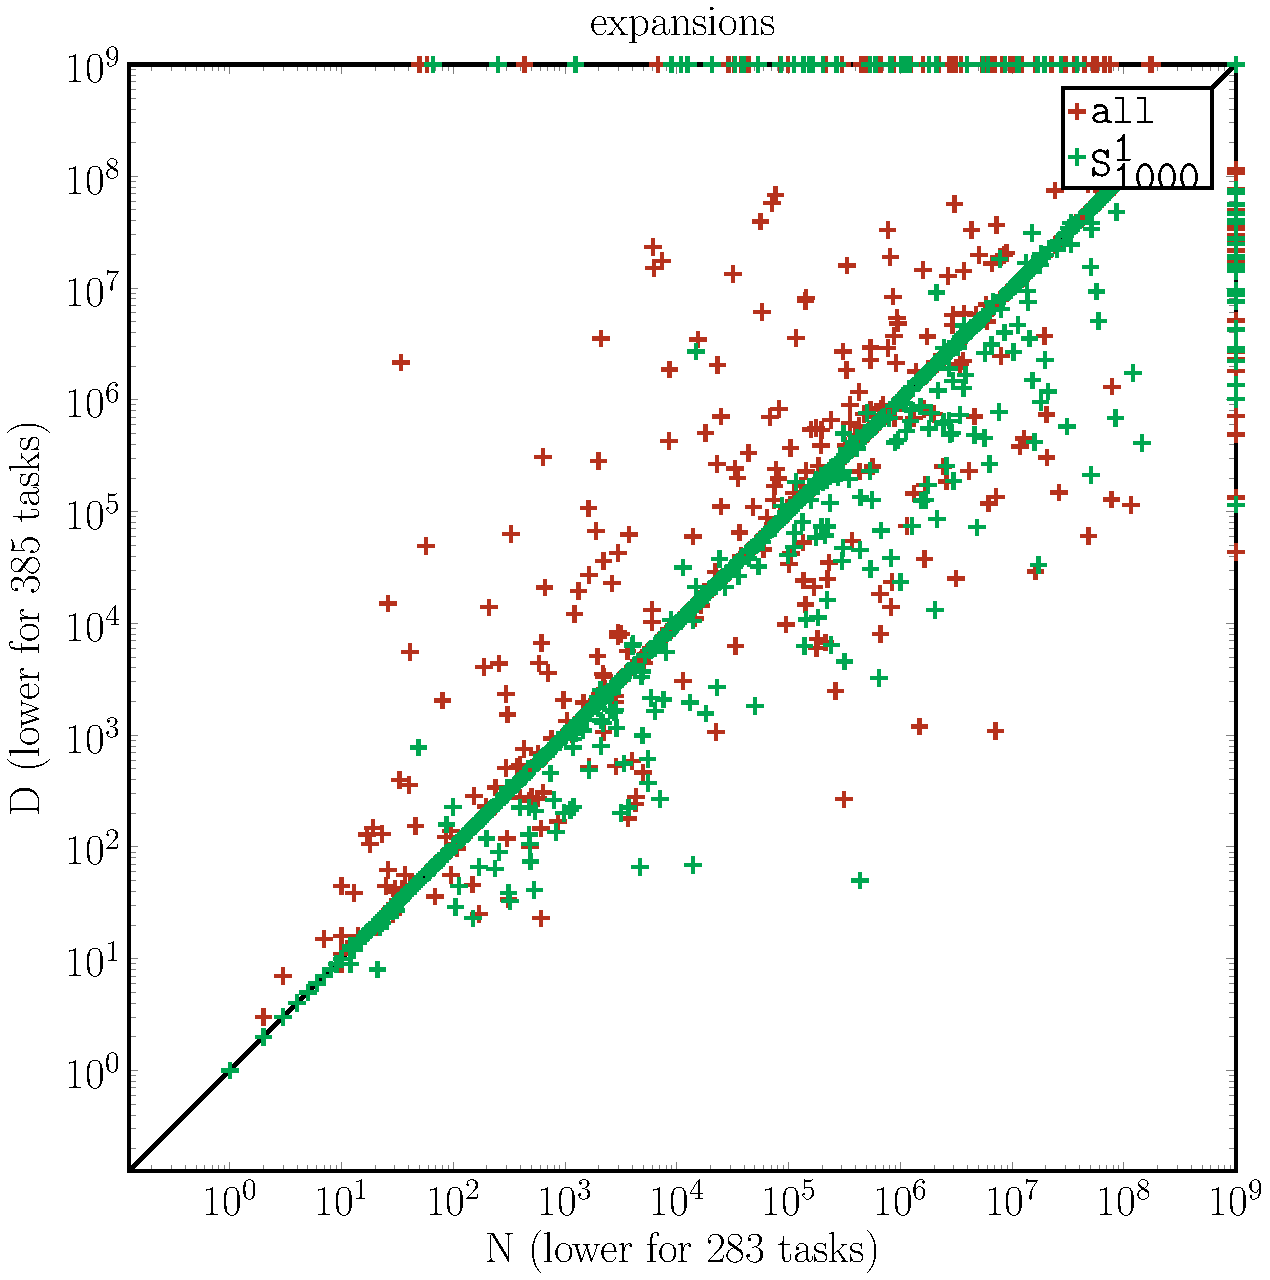
\includegraphics[width=0.45\textwidth]{N_D_exp}
        \end{figure}
    \end{frame}

    \section{Optimization Functions}
    \begin{frame}[c]{Mutex Based Optimization Functions}
        \begin{definition}[Mutex Based Optimization Function]
            \[\mathrm{opt}^k_\mathcal{M}=\sum_{f=\langle V,v \rangle\in\mathcal{F}}\frac{\mathcal{C}_f^k(\mathcal{M})}{\sum_{f'\in\mathcal{F}_V}\mathcal{C}_{f'}^k(\mathcal{M})}\mathtt{P}(f)\]
        \end{definition}

        \begin{definition}[Mutex Based Ensemble Optimization Function]
            \[\mathrm{opt}^{t,k}_\mathcal{M}=\sum_{f=\langle V,v \rangle\in\mathcal{F}}\frac{\mathcal{K}^k_f(\mathcal{M}, t)}{\sum_{f'\in\mathcal{F}_V}\mathcal{K}^k_f(\mathcal{M}, t)}\mathtt{P}(f)\]
        \end{definition}
    \end{frame}

    \begin{frame}[c]{Mutex Based Optimization Functions: Results}
        \begin{table}[ht!]
            \centering
            \begin{tabular}{|r|c|c|c|}
                \hline
                & \textbf{\texttt{all-N}} & \textbf{$\texttt{M}_{\texttt{1}}$\texttt{-D}} & \textbf{$\texttt{J}_{\texttt{1}}^{\texttt{10}}$\texttt{-D}} \\
                \hline \hline
                \textbf{Coverage}       & 929 & 900 & 922 \\ \hline
                \textbf{Expansions}     & 10244 & 8297 & 6197\\ \hline
                \textbf{Total Time}     & 0.29 & 0.59 & 1.02 \\ \hline
                \textbf{Search Time}    & 0.23 & 0.20 & 0.89 \\ \hline
            \end{tabular}
        \end{table}
    \end{frame}

    \section{Additional Constraints}
    \begin{frame}[c]{Additional Constraints}
        \begin{definition}[Additional Constraint]
            \[\sum_{f\in s}\mathtt{P}(f)=h^\mathtt{P}(s)\]
        \end{definition}
    \end{frame}

    \begin{frame}[c]{Additional Constraints: Results}
        \begin{columns}
            \column{.5\textwidth}
            \begin{figure}
                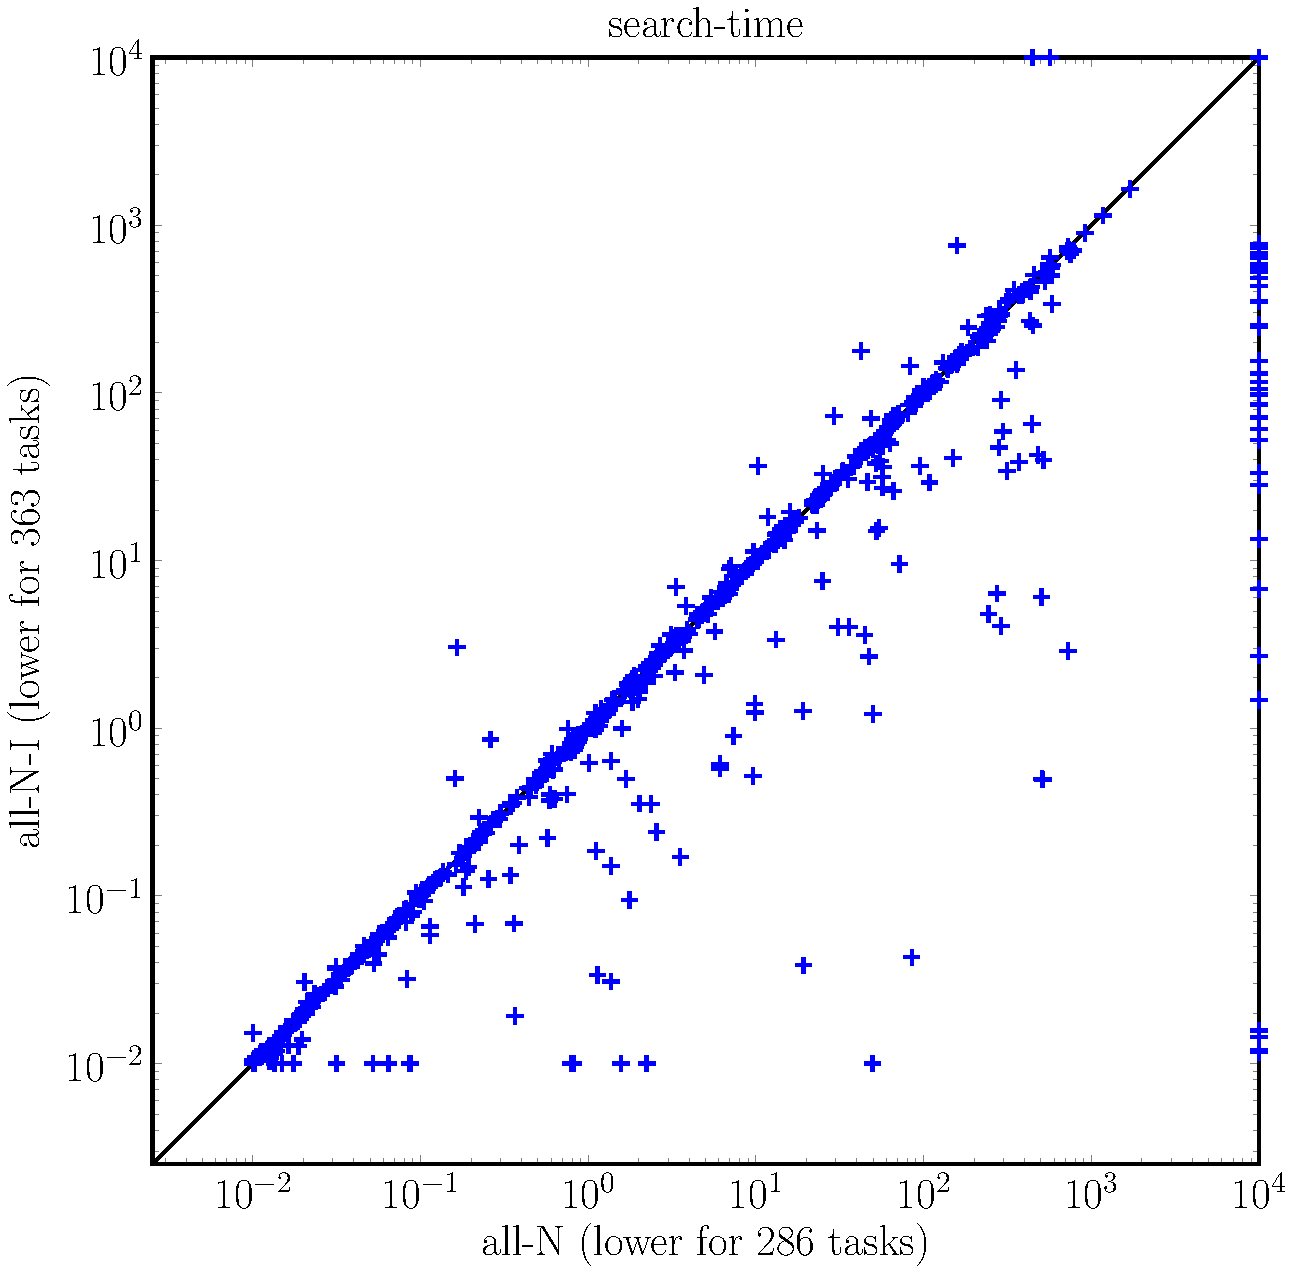
\includegraphics[width=0.9\textwidth]{all_I_search}
            \end{figure}

            \column{.5\textwidth}
            \begin{figure}
                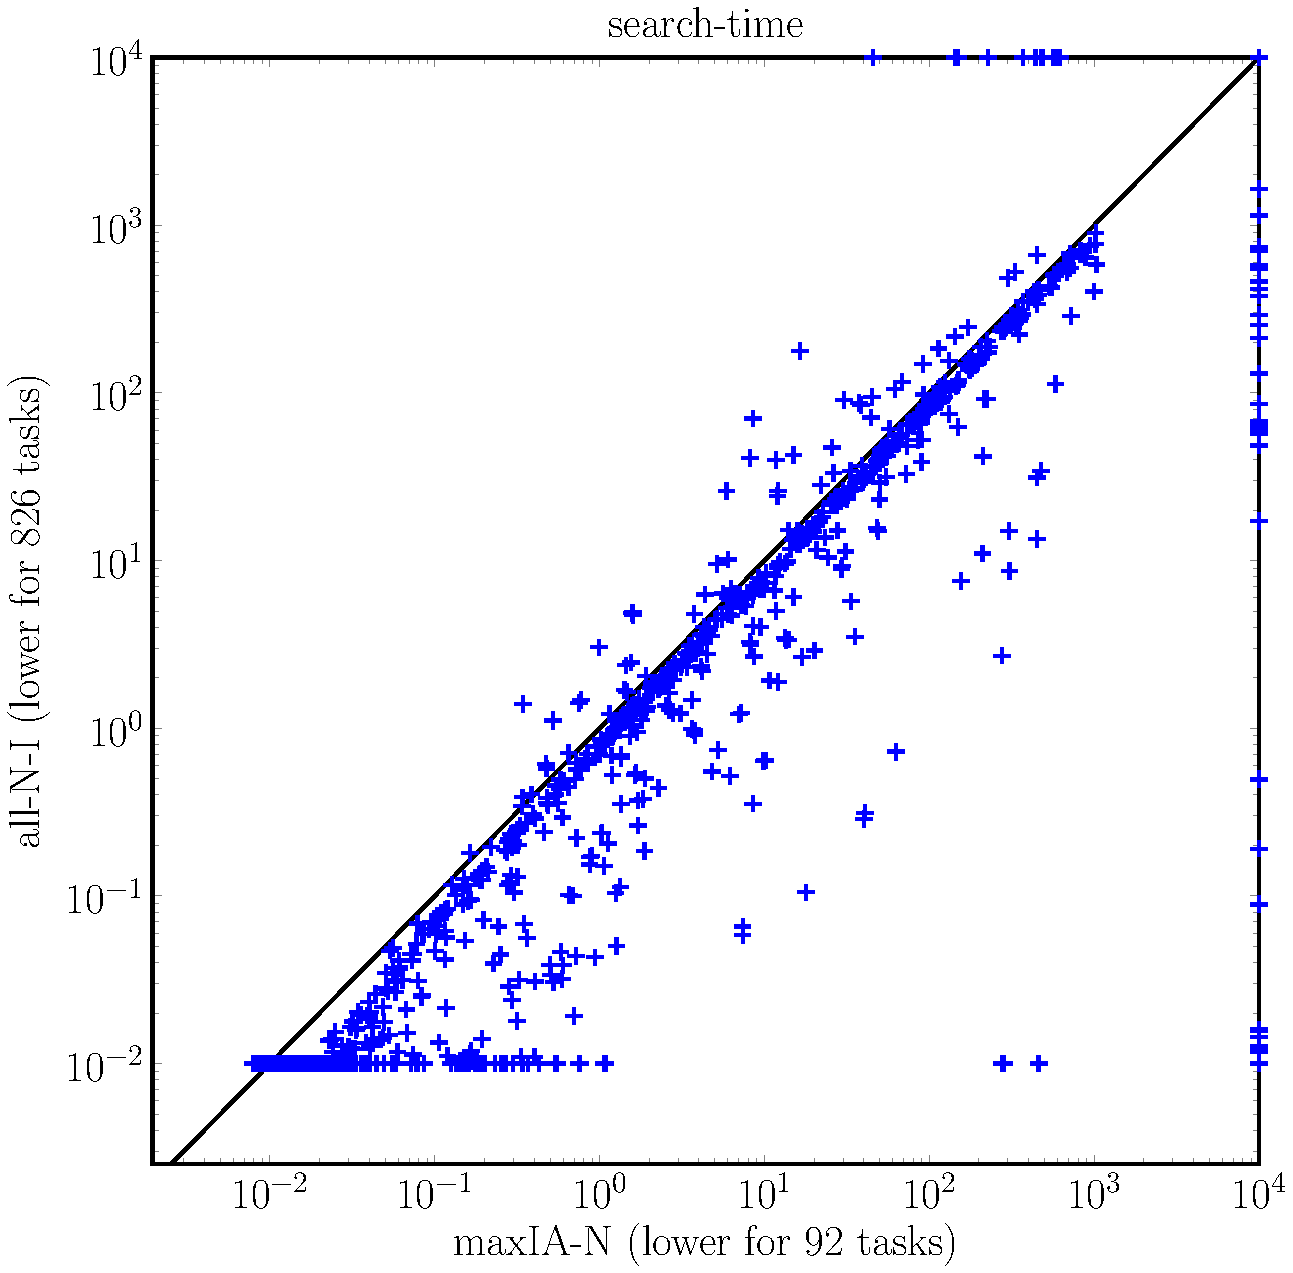
\includegraphics[width=0.9\textwidth]{all_max_search}
            \end{figure}
        \end{columns}
    \end{frame}

    \section{Conclusion}
    \begin{frame}[c]{Conclusion}
        \begin{itemize}
            \item Too computationally expensive
            \item Additional constraints good
        \end{itemize}
    \end{frame}

    \begin{frame}[t,plain]
        \lastpage{{\usebeamerfont{title} Questions?}\\[5ex]
        salo.mueller@unibas.ch}
    \end{frame}

    \backupbegin

    \begin{frame}[c]{Max(all, init)}
        \begin{table}[h!]
            \center
            \begin{tabular}{|r|c|c|c|c|c|c|}
                \hline
                & \textbf{\texttt{all-N}} & \textbf{\texttt{all-N-I}} & \textbf{\texttt{all-N-I-WP}} & \textbf{\texttt{max-N}} & \textbf{\texttt{max-N-WP}} & \textbf{\texttt{max-N-I}} \\
                \hline \hline
                \textbf{Coverage}       & 929 & \textbf{965} & \textbf{965} & 948 & 957 & 958 \\ \hline
                \textbf{Expansions}     & 53184 & 49875 & 40519 & 38914 & 36556 & \textbf{35804} \\ \hline
                \textbf{Total Time}     & 1.12 & \textbf{0.98} & 1.00 & 1.13 & 1.13 & 1.10 \\ \hline
                \textbf{Search Time}    & 0.90 & \textbf{0.75} & 0.77 & 0.85 & 1.11 & 0.83 \\ \hline
                \textbf{Out of Memory}  & 870 & 837 & \textbf{835} & 854 & 843 & 843 \\ \hline
                \textbf{Out of Time}    & 11 & \textbf{8} & 10 & \textbf{8} & 10 & 9 \\ \hline
            \end{tabular}
        \end{table}
    \end{frame}

    \begin{frame}[c]{Standard Potential Heuristics}
        \begin{table}[h!]
            \center
            \begin{tabular}{|r|c|c|c|c|c|c|c|}
                \hline
                & \textbf{\texttt{lmc}} & \textbf{\texttt{all-N}} & \textbf{\texttt{init-N}} & \textbf{\texttt{max-N}} & \textbf{\texttt{div-N}} & \textbf{$\texttt{S}_{\texttt{1}}^{\texttt{100}}$\texttt{-N}} & \textbf{$\texttt{S}_{\texttt{1000}}^{\texttt{1}}$\texttt{-N}} \\
                \hline \hline
                \textbf{Coverage}       & 958 & 929 & 891 & 948 & \textbf{963}  & 945 & 961   \\ \hline
                \textbf{Expansions}     & \textbf{1287} & 10244 & 22415 & 8270 & 6904 & 7181 & 9238  \\ \hline
                \textbf{Total Time}     & 0.57 & \textbf{0.29} & 0.54 & 0.33 & 0.74 & 0.94 & 0.33  \\ \hline
                \textbf{Search Time}    & 0.52 & 0.23 & 0.43 & 0.24 & 0.74 & 0.94 & \textbf{0.22}  \\ \hline
                \textbf{Out of Memory}  & \textbf{0}    & 870 & 911 & 854 & 623 & 170 & 844   \\ \hline
                \textbf{Out of Time}    & 852 & 11 & 8 & 8 & 224 & 695 & \textbf{5}     \\ \hline
            \end{tabular}
        \end{table}
    \end{frame}

    \begin{frame}[c]{Strengthened Constraints}
        \begin{table}[h!]
            \center
            \begin{tabular}{|r|c|c|c|c|c|c|}
                \hline
                & \textbf{\texttt{all-D}} & \textbf{\texttt{init-D}} & \textbf{\texttt{max-D}} & \textbf{\texttt{div-D}} & \textbf{$\texttt{S}_{\texttt{1}}^{\texttt{100}}$\texttt{-D}}& \textbf{$\texttt{S}_{\texttt{1000}}^{\texttt{1}}$\texttt{-D}}\\
                \hline \hline
                \textbf{Coverage}       & 879 & 881 & 932 & 837 & 853 & \textbf{952}  \\ \hline
                \textbf{Expansions}     & 12101 & 18964 & 7863 & \textbf{5269} & 5503 & 7697          \\ \hline
                \textbf{Total Time}     & 0.68 & 0.90 & 0.84 & 4.18 & 3.29 & \textbf{0.64} \\ \hline
                \textbf{Search Time}    & 0.27 & 0.39 & 0.24 & \textbf{0.19} & 0.31 & \textbf{0.19} \\ \hline
                \textbf{Out of Memory}  & 824 & 824 & 770 & 560 & \textbf{273}  & 726           \\ \hline
                \textbf{Out of Time}    & 75 & \textbf{73}   & 76 & 381 & 652 & 100           \\ \hline
            \end{tabular}
        \end{table}
    \end{frame}

    \begin{frame}[c]{Strengthened Optimization Functions}
        \begin{table}[h!]
            \center
            \begin{tabular}{|r|c|c|c|c|c|c|c|c|c|}
                \hline
                & \textbf{$\texttt{M}_{\texttt{1}}$\texttt{-D}} & \textbf{$\texttt{M}_{\texttt{2}}$\texttt{-D}} & \textbf{$\texttt{K}_{\texttt{1}}^{\texttt{10}}$\texttt{-D}} & \textbf{$\texttt{K}_{\texttt{2}}^{\texttt{10}}$\texttt{-D}} & \textbf{$\texttt{L}_{\texttt{1}}^{\texttt{10}}$\texttt{-D}} & \textbf{$\texttt{L}_{\texttt{2}}^{\texttt{10}}$\texttt{-D}} & \textbf{$\texttt{J}_{\texttt{1}}^{\texttt{10}}$\texttt{-D}} & \textbf{$\texttt{J}_{\texttt{2}}^{\texttt{10}}$\texttt{-D}}\\
                \hline \hline
                \textbf{Coverage}       & 900 & 859 & 911 & 831 & 921 & 840 & \textbf{922}  & 845   \\ \hline
                \textbf{Expansions}     & 8297 & 8240 & 6790 & 6847 & 6126 & 6273 & 6197 & \textbf{6039} \\ \hline
                \textbf{Total Time}     & \textbf{0.59} & 1.23 & 0.89 & 4.23 & 0.99 & 3.93 & 1.02 & 3.20  \\ \hline
                \textbf{Search Time}    & \textbf{0.20} & \textbf{0.20} & 0.86 & 4.08 & 0.86 & 3.78 & 0.89 & 3.04  \\ \hline
                \textbf{Out of Memory}  & 802 & 726 & 714 & 608 & 691 & 589 & 677 & \textbf{586}   \\ \hline
                \textbf{Out of Time}    & \textbf{77}   & 203 & 155 & 351 & 169 & 364 & 193 & 364   \\ \hline
            \end{tabular}
        \end{table}
    \end{frame}

    \begin{frame}[c]{Additional Constraint on the Initial State}
        \begin{table}[h!]
            \center
            \begin{tabular}{|r|c|c|c|c|c|}
                \hline
                & \textbf{\texttt{all-N-I}} & \textbf{\texttt{div-N-I}} & \textbf{$\texttt{S}_{\texttt{1000}}^{\texttt{1}}$\texttt{-N-I}} & \textbf{$\texttt{M}_{\texttt{1}}$\texttt{-D-I}} & \textbf{$\texttt{M}_{\texttt{2}}$\texttt{-D-I}} \\
                \hline \hline
                \textbf{Coverage}       & \textbf{965}  & 956 & 963 & 950 & 906 \\ \hline
                \textbf{Expansions}     & 8532 & 7741 & 9040 & 6585 & \textbf{6561} \\ \hline
                \textbf{Total Time}     & \textbf{0.27} & 0.70 & 0.33 & 0.60 & 1.21 \\ \hline
                \textbf{Search Time}    & 0.21 & 0.70 & 0.21 & \textbf{0.17} & \textbf{0.17} \\ \hline
                \textbf{Out of Memory}  & 837 & 716 & 843 & 729 & \textbf{705} \\ \hline
                \textbf{Out of Time}    & 8 & 127 & \textbf{4}& 115 & 183 \\ \hline
            \end{tabular}
        \end{table}
    \end{frame}

    \begin{frame}[c]{Additional Constraints on Random States}
        \begin{table}[h!]
            \center
            \begin{tabular}{|r|c|c|c|c|}
                \hline
                & \textbf{\texttt{all-N-R}} & \textbf{\texttt{init-N-R}} &\textbf{\texttt{div-N-R}} & \textbf{$\texttt{M}_{\texttt{2}}$\texttt{-D-R}} \\
                \hline \hline
                \textbf{Coverage}       & \textbf{930}  & 898 & 905 & 863 \\ \hline
                \textbf{Expansions}     & 11672 & 16182 & 11306 & \textbf{9190} \\ \hline
                \textbf{Total Time}     & \textbf{0.35} & 0.44 & 0.76 & 1.51 \\ \hline
                \textbf{Search Time}    & \textbf{0.34} & 0.44 & 0.76 & 1.37 \\ \hline
                \textbf{Out of Memory}  & 858 & 899 & 798 & \textbf{728} \\ \hline
                \textbf{Out of Time}    & 16 & \textbf{11}   & 105 & 205 \\ \hline
            \end{tabular}
        \end{table}
    \end{frame}

    \begin{frame}[c]{Mutex Based Optimization Functions}
        \begin{definition}[Mutex Based Optimization Function]
            \[\mathcal{C}_f^k(\mathcal{M}) = \sum_{p\in\mathcal{P}_k^{\{f\}}}\prod_{V\in\mathcal{V}} |F_V\setminus\mathcal{M}_p|\]
        \end{definition}

        \begin{definition}[Mutex Based Ensemble Optimization Function]
            \[\mathcal{K}^k_f(\mathcal{M}, t) = \sum_{p\in\mathcal{P}^{t\cup\{f\}}_{|t|+k}}\prod_{V\in\mathcal{V}}|\mathcal{F}\setminus\mathcal{M}_p|\]
        \end{definition}
    \end{frame}

    \begin{frame}[c]{LP Constraints}
        \begin{theorem}
            \label{theorem:theorem 5} % Theorem 6
            Let $\Pi = \langle \mathcal{V}, \mathcal{O}, I, G \rangle$ denote a planning task, $\mathtt{P}$ a
            potential function, and for every operator $o\in\mathcal{O}$, let
            $\mathrm{pre}^*(o)=\{\langle V, \mathrm{pre}(o)[V]\rangle |V\in \mathrm{vars(pre}(o))\cap\mathrm{vars(eff}(o))\}$ and
            $\mathrm{vars}^*(o)=\mathrm{vars(eff}(o))\setminus\mathrm{vars(pre}(o))$. If
            \begin{equation}
                \sum_{f\in G}\mathtt{P}(f)+\sum_{V\in\mathcal{V}\setminus\mathrm{vars}(G)}\max_{f\in\mathcal{F}_V}\mathtt{P}(f)\leq0\label{eq:1}
            \end{equation}
            and for every operator $o\in\mathcal{O}$ it holds that
            \begin{equation}
                \sum_{f\in\mathrm{pre}^*(o)}\mathtt{P}(f)+\sum_{V\in\mathrm{vars}^*(o)}\max_{f\in\mathcal{F}_V}\mathtt{P}(f)-\sum_{f\in\mathrm{eff}(o)}\mathtt{P}(f)\leq c(o)\label{eq:2}
            \end{equation}
            then the potential heuristic for $\mathtt{P}$ is admissible.
        \end{theorem}


    \end{frame}

    \backupend

\end{document}

